\documentclass[12pt, oneside, a4paper, dvipdfm fleqn]{article}
\usepackage{natbib}
	    
\usepackage[utf8x]{inputenc}
\usepackage[brazil]{babel}
\usepackage{indentfirst}		% Indenta o primeiro parágrafo de cada seção.
\usepackage{nomencl} 			% Lista de simbolos
\usepackage{color}				% Controle das cores
\usepackage{graphicx}			% Inclusão de gráficos
\usepackage{microtype} 			% para melhorias de justificação
\usepackage[dvipsnames]{xcolor,colortbl}
\usepackage{adjustbox}
\usepackage{svg}
\usepackage{hyperref}
\usepackage{graphicx,color}
\usepackage{graphicx,url}

\usepackage{listings}
\usepackage{caption,multicol,booktabs,array}

\hypersetup{
	colorlinks = true, % false: boxed links; true: colored links
	linkcolor = orange, % cor para links
	citecolor = orange, % cor para links em bibliografia
	urlcolor= orange, % cor da url na bibliografia
	}
\usepackage{float}
 
\usepackage{amssymb}
\usepackage{amsmath}

\usepackage{lipsum}			
\usepackage{verbatim}
\usepackage{setspace}
\usepackage{listing}

\definecolor{darkgray}{rgb}{.4,.4,.4}
\definecolor{purple}{rgb}{0.65, 0.12, 0.82}
\definecolor{azulzinho}{rgb}{0.36, 0.54, 0.66}
\lstdefinelanguage{WSML}{
keywords={ontology, wsmlVariant, namespace, ofType, subConceptOf, concept, axiom, hasValue, definedBy, memberOf, instance, relation, relationInstance,  and},
keywordstyle=\color{purple}\bfseries,
ndkeywords={class, export, boolean, throw, implements, import, this,x,?},
ndkeywordstyle=\color{red}\bfseries,
identifierstyle=\color{black},
sensitive=false,
comment=[l]{//},
morecomment=[s]{"}{"},
commentstyle=\color{blue}\ttfamily,
stringstyle=\color{azulzinho}\ttfamily,
morestring=[b]',
morestring=[b]"
}

\lstset{
language=WSML,
extendedchars=true,
frame = single,
basicstyle=\scriptsize\ttfamily,
showstringspaces=false,
showspaces=false,
numbers=left,
numberstyle=\scriptsize,
numbersep=9pt,
xleftmargin=.05\textwidth, 
xrightmargin=.05\textwidth,
tabsize=2,
breaklines=true,
showtabs=false,
captionpos=b
}


\doublespacing
%\onehalfspacing

\RequirePackage[a4paper,top=3.5cm,left=3cm,right=3cm,bottom=2.5cm]{geometry}

\parindent 0em

% O tamanho do parágrafo é dado por:
\setlength{\parindent}{1.3cm}

% Controle do espaçamento entre um parágrafo e outro:
%\setlength{\parskip}{0.2cm}  % tente também \onelineskip
\interfootnotelinepenalty=10000 
\begin{document}

\noindent\textbf{Universidade Federal de Sergipe} \\
\textbf{Campus Prof. Alberto Carvalho}   \\
\textbf{Departamento de Sistemas de Informação} \\

\noindent\textbf{Título do Projeto}\\
\textit {Lixeira Inteligente: }Um sistema eficiente para reciclagem de lixo \\
\noindent\textbf{Orientador:} \textit{Prof. Dr. André Luis Meneses Silva} \\
\textbf{Alunos:} Arlene De Almeida Pereira Siqueira, Camila Fontes Santos, Laila Esterfane Dos Santos Valença, Marlysson Silva Dantas, Miguel Ferreira França e Vinicius Lima Santos \\


% ----------------------
% ELEMENTOS PRE-TEXTUAIS
% ----------------------

%-------------------

% -------------------
% ELEMENTOS TEXTUAIS
% -------------------

\section{Introdução} \label{sec:Intro}
A gestão eficiente de resíduos sólidos é um desafio crescente nas sociedades modernas. A busca por soluções inovadoras que tornem esse processo mais prático e sustentável tem conduzido a avanços tecnológicos em várias áreas.\cite{sensor}\footnote{Referêcia detalhada sobre sensor utilizado.} e com o objetivo de desenvolver
de uma lixeira automática equipada com sensores  e mecanismos de automação que visem otimizar a coleta e a limpeza de lixeiras públicas este trabalho foi desenvolvido.

A proposta se baseia em um sistema composto por uma série de etapas coordenadas, com o objetivo de melhorar a eficiência da coleta de resíduos, garantindo que a lixeira esteja sempre pronta para receber novos resíduos de maneira higiênica e eficaz. Cada etapa do processo é cuidadosamente planejada e automatizada, permitindo que a lixeira realize a limpeza e a preparação para a próxima coleta de maneira automatica.

A lixeira automática traz consigo um novo meio de explorar a sustentabilidade das grandes cidades e da sua interação com o meio ambiente, no entanto surge a necessidade de implementar na sua automação aparelhos que tornem essa automatização possível, sendo esses componentes, conjuntos de aparelhos que trabalham de maneira uniforme e que atingem o esperado, sendo a limpeza e a lacração automática da sacola de lixo. Dito isso, a Lixeira Automática é equipada com sensores avançados, atuadores e um sistema de controle baseado na plataforma Raspberry Pi \cite{raspberry}\footnote{Referência detalhada sobre Raspberry Pi.}, tornando-a capaz de detectar o nível de enchimento da lixeira, a presença de uma bolsa de resíduos, e realizar uma sequência de ações automáticas, incluindo a limpeza da lixeira e o selamento da sacola, tornando-a pronta para o próximo ciclo de coleta.

Este trabalho aborda detalhadamente o projeto, implementação e avaliação da Lixeira Automática. Ele descreve o \textit{hardware} e \textit{software} envolvidos, a lógica de automação, a calibração de sensores, a eficiência energética, os testes práticos, a sustentabilidade e o impacto social do sistema. Além disso, compara a lixeira automática com as soluções tradicionais de coleta de resíduos em termos de eficiência, custo e sustentabilidade.

O objetivo deste projeto é proporcionar uma contribuição significativa para a gestão de resíduos urbanos, criando um sistema inovador que promova a limpeza, a sustentabilidade e a qualidade de vida nas áreas urbanas. Ao explorar as potencialidades da tecnologia, este trabalho visa inspirar futuras soluções criativas e eficientes para os desafios urbanos contemporâneos de gestão de resíduos. Na próxima seção, apresentamos os objetivos gerais e específicos desta proposta.



\subsection{Objetivos do Projeto} \label{sec:objProj}

O objetivo geral dessa proposta consiste em criar uma solução computacional que combine componentes de \textit{hardware} e \textit{software}, com a finalidade de contribuir para a prática mais eficiente da reciclagem de resíduos a nível global.

Como objetivos específicos, temos:

\begin{itemize}
    \item Realizar levantamentos bibliográficos sobre sensores, microcomputadores, seleção dos componentes necessários;
    \item Desenvolvimento de código de programação para microcontrolador, de modo que controle todos os aspectos do sistema, incluindo sensores e toda a lógica de automação;
    \item Desenvolver e implementar com sucesso a sequência de ações automáticas que ocorrem quando a lixeira está cheia, incluindo a limpeza e o selamento da sacola;
    \item Realizar uma análise de custos para avaliar a viabilidade financeira do
projeto, incluindo custos de construção e operação;
    \item Avaliar o impacto social da lixeira inteligente, incluindo sua contribuição para a manutenção de ambientes urbanos limpos e para a qualidade de vida dos moradores.
\end{itemize}

\subsection{Estrutura da Proposta}
Esta proposta adota a seguinte estrutura organizacional: a Seção 2 delineia o Referencial Teórico, destacando as ferramentas de automação da Lixeira Inteligente. A seguir, na Seção 3, são expostos os Trabalhos Relacionados, abordando pesquisas correlatas a esta proposta. Na Seção 4, é esboçada a Metodologia, contemplando as etapas do projeto, os recursos a serem empregados e a visão do resultado almejado. Por último, a Seção 5 apresenta as Conclusões.
\section{Referencial Teórico} \label{sec:refTeorico}
Nesta seção, serão abordados conceitos fundamentais para a compreensão dessa proposta, são eles: Inteligência Artificial, Internet das Coisas (IoT), Microcomputador, Servo Motor, Sensor Ultrassônico, Válvulas Selenóide e bombeamento de água. 

\subsection{Inteligência Artificial}
A inteligência artificial (IA), conforme definido pela \cite{ia}, já é parte da tecnologia moderna, pois, ela torna possível o aprendizado de máquina e a tomada de decisões, em uma velocidade e eficiência superiores aos seres humanos.

A IA desempenha um papel fundamental em diversos aspectos de nossa vida cotidiana, desde assistentes virtuais presentes em nossos smartphones até carros autônomos que podem navegar por conta própria. Pense em ter um amigo digital que compreende suas palavras, responde às suas perguntas e até mesmo antecipa suas necessidades futuras. A IA é essa amiga digital, e sua habilidade de aprender com a experiência a torna cada vez mais inteligente com o tempo.

À medida que a IA continua a evoluir nos apresenta novas formas de   tornar nossas vidas mais convenientes e eficazes. No entanto, também suscita questões cruciais relacionadas à privacidade e ética que exigem uma atenção cuidadosa. Em resumo, a inteligência artificial é uma tecnologia que está transformando nosso mundo de maneiras fascinantes e revolucionárias, tal como definiu \cite{John}, o pai da IA, como "a ciência e a engenharia de criar máquinas inteligentes".


\subsection{Internet das Coisas (IoT)}
A Internet das Coisas (IoT), conforme descrita pela \cite{iot}, representa uma revolução tecnológica que viabiliza a interconexão de objetos em nosso cotidiano, conferindo-lhes a capacidade de comunicação e coleta de dados. Em termos simples, trata-se da habilidade de dispositivos comuns, incluindo eletrodomésticos, sensores, veículos e até mesmo roupas, conectarem-se à internet e compartilharem informações entre si.
=90
Essa rede de objetos inteligentes tem a capacidade de coletar, analisar e compartilhar dados relevantes, contribuindo para aprimorar a eficiência, automação e comodidade nas atividades do dia a dia. Um exemplo prático é a capacidade de um termostato ajustar a temperatura da sua residência com base nas informações de previsão do tempo ou de uma pulseira que monitora sua saúde e envia dados ao seu médico. Em resumo, a IoT representa um avanço tecnológico que torna nossos objetos cotidianos mais inteligentes e interconectados, com o propósito de melhorar nossas vidas.

\subsection{Single Board Computer}Single Board Computer
Um microcomputador, como descrito no site oficial do \cite{raspberry}, é um tipo de computador pessoal notavelmente compacto, projetado para executar tarefas diversificadas e específicas. Estes dispositivos, frequentemente do tamanho de um cartão de crédito, ou ainda menores, são equipados com componentes de processamento, memória e conectividade que lhes permitem desempenhar uma ampla variedade de funções.

 Apesar de sem enquardar perfeitamente na definição de acima, o Raspberry Pi na verdade é um exemplo de SBC (Single Board Computer), que ganhou ampla popularidade. O SBC oferece capacidades de processamento, entrada/saída e conectividade, bem como a capacidade de executar sistemas operacionais, o que possibilita aos usuários a realização de diversas tarefas, desde programação e navegação na web até o controle de dispositivos eletrônicos.

A característica distintiva dos microcomputadores reside em sua portabilidade e versatilidade. Eles encontram aplicação em projetos de automação residencial, sistemas de monitoramento, servidores domésticos e muito mais. A acessibilidade e a facilidade de programação tornam os microcomputadores uma ferramenta valiosa tanto para entusiastas quanto para desenvolvedores e educadores interessados em explorar o campo da eletrônica e da computação.

Em resumo, um microcomputador é uma categoria de dispositivos eletrônicos compactos e versáteis, que oferece uma plataforma para experimentação, aprendizado e desenvolvimento de projetos em diversas áreas, desde eletrônica até automação e computação.

\subsubsection{Raspberry Pi}
 A Figura 1 apresenta o Raspberry Pi, conforme explicado no site oficial do \cite{raspberry}, é um SBC de placa única pois todos os principais componentes de um computador, como processador, memória e conectividade, estão integrados em uma única placa, proporcionando funcionalidade completa em um espaço compacto, ao qual se destaca pela sua versatilidade e facilidade de uso. Embora seja do tamanho de um cartão de crédito, este dispositivo é equipado com recursos de processamento e conectividade que o tornam incrivelmente versátil.

O Raspberry Pi é um sistema completo, com portas USB para conexão de teclado, mouse e outros dispositivos, bem como portas HDMI para conexão a um monitor ou TV. Além disso, ele possui portas GPIO (Entrada/Saída de Propósito Geral) que possibilitam a interação com sensores, LEDs e outros dispositivos eletrônicos.

O Raspberry Pi é capaz de executar sistemas operacionais, como o Raspberry Pi OS, que podem ser instalados em um cartão microSD. Isso possibilita a execução de uma ampla variedade de aplicativos e a realização de tarefas, como navegação na web, programação, reprodução de mídia e até mesmo a criação de servidores.

Este SBC é frequentemente utilizado em projetos de automação residencial, robótica, educação em programação, servidores domésticos e muito mais. Sua acessibilidade e recursos tornam o Raspberry Pi uma plataforma ideal para explorar a computação, eletrônica e desenvolvimento de projetos.

Ou seja, o Raspberry Pi é um SBC de baixo custo que oferece uma ampla gama de possibilidades para aprendizado e desenvolvimento de projetos, tornando-o uma ferramenta ideal para explorar o mundo da tecnologia de forma criativa e prática.

 \begin{figure}[H]
    \caption{Raspberry Pi}
    \label{fig:raspberryImagem}
    \begin{center}
        
        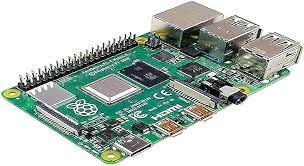
\includegraphics[scale=1]{Textuais/imagens/raspberry.png}
        
        Fonte:  Aliexpress
    \end{center}
\end{figure}

\subsection{Servo Motor}
Na Figura 2 temos um exemplo de servo motor, que é definido no site  \cite{servomotor} como um dispositivo eletromecânico projetado para controlar a posição de uma haste ou alavanca em resposta a um sinal de controle. Esse tipo de dispositivo é amplamente empregado em diversas aplicações que demandam movimentos precisos, como na área de robótica, sistemas de automação industrial e modelagem de aeromodelismo. O servo motor é reconhecido por sua habilidade em girar ou mover-se até uma posição específica, obedecendo comandos precisos, tornando-o uma escolha proeminente para o controle de movimentos de alta precisão.

O funcionamento do servo motor é fundamentado em um sistema interno de feedback. Ele consiste de um motor elétrico, um conjunto de engrenagens e, normalmente, um dispositivo de feedback, que frequentemente é um potenciômetro. Quando um sinal de controle é aplicado ao servo motor, o motor se movimenta com o intuito de posicionar a haste ou alavanca na direção desejada. O dispositivo de feedback mantém constante monitoramento da posição atual e transmite informações ao controlador do servo motor, permitindo-lhe realizar ajustes precisos para manter a posição desejada.

A capacidade intrínseca de controle preciso faz do servo motor a escolha ideal para aplicações que requerem movimentos angulares específicos, como o ajuste da posição de um braço robótico ou a direção das rodas de um veículo autônomo. Além disso, os servo motores são extensivamente aplicados na área de aeromodelismo, onde controlam superfícies como lemes e ailerons.

Resumindo, o servo motor é um dispositivo eletromecânico projetado para efetuar um controle preciso da posição de uma haste ou alavanca em resposta a comandos. Essa característica o torna fundamental em diversas aplicações que exigem movimentos controlados e precisos.

 \begin{figure}[H]
    \caption{Servo Motor}
    \label{fig:servomotorImagem}
    \begin{center}
        
        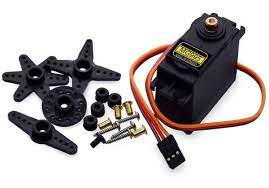
\includegraphics[scale=1]{Textuais/imagens/servomotor.png}
        
        Fonte: Mercado Livre
    \end{center}
\end{figure}

\subsection{Válvula Solenoide}
Uma válvula solenoide, conforme detalhado no manual de instalação de válvulas solenoide da \cite{valvula} e apresentado na Figura 3, é um dispositivo eletromecânico projetado para regular o fluxo de fluidos, como líquidos ou gases, em sistemas de tubulação. A operação desse dispositivo é baseada nos princípios da eletricidade e do magnetismo. A componente essencial da válvula solenoide é uma bobina eletromagnética que, quando alimentada eletricamente, cria um campo magnético. Esse campo magnético age sobre uma haste móvel, conhecida como núcleo, localizada no interior da bobina. Quando o núcleo é atraído pelo campo magnético, ele movimenta um obturador ou diafragma, resultando na abertura ou fechamento da passagem do fluido através da válvula.

As válvulas solenoides encontram uma ampla gama de aplicações, abrangendo desde sistemas de irrigação e controle de fluidos industriais até eletrodomésticos, como máquinas de lavar e cafeteiras. Elas proporcionam uma forma eficaz e precisa de gerenciar o fluxo de fluidos, sendo ativadas por meio de sinais elétricos. Isso permite que as válvulas solenoides sejam controladas remotamente e automatizadas conforme as exigências do sistema.

Resumidamente, uma válvula solenoide é um dispositivo eletromecânico que regula o fluxo de líquidos ou gases em sistemas, realizando tal controle por meio da ativação de uma bobina eletromagnética. Sua versatilidade e precisão a tornam uma solução comum em uma variedade de aplicações, assegurando um controle eficiente e confiável de fluidos em diversos sistemas.

 \begin{figure}[H]
    \caption{Válvula Selenóide}
    \label{fig:valvulaImagem}
    \begin{center}
        
        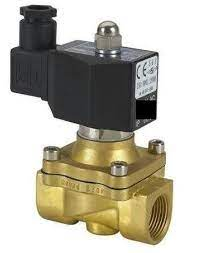
\includegraphics[scale=1]{Textuais/imagens/valvula.png}
        
        Fonte: Amazon
    \end{center}
\end{figure}

\subsection{Bombeamento de água}
Sistema de Bombeamento de Água: O sistema de bombeamento de água, conforme detalhado no site da \cite{bomba}, a mini bomba de agua 12V RS385 foi projetada com foco na prototipagem e é especialmente adequada para aplicações em automação residencial (domótica) e protótipos de robótica baseados em microcontroladores populares, como Arduino e Raspberry Pi. Figura 4 é um exemplo de bomba de água.

Com seu motor de tamanho apropriado, esta bomba é capaz de impulsionar uma quantidade de água significativa, variando de 1500ml a 2000ml por minuto. Sua eficiência e precisão se destacam, particularmente quando utilizada em conjunto com dispositivos como o Arduino.

Esta bomba encontra aplicação em uma variedade de projetos, incluindo carrinhos ou robôs de combate a incêndios, robôs hidráulicos e sistemas de irrigação automática, com foco na automação residencial. Sua versatilidade permite que sua criatividade determine sua aplicação final.

\begin{figure}[H]
    \caption{Bomba de água}
    \label{fig:bombaImagem}
    \begin{center}
        
        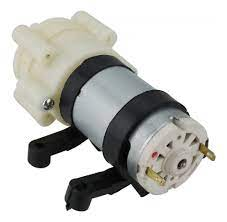
\includegraphics[scale=1]{Textuais/imagens/bomba.png}
        
        Fonte: Mercadolivre
    \end{center}
\end{figure}

\subsection{Sensor Ultrassônico HC-SR04} O sensor ultrassônico HC-SR04, descrito no \cite{sensor} e apresentado na Figura 5, é um dispositivo que utiliza ondas sonoras de alta frequência para medir distâncias. Funciona emitindo um sinal sonoro inaudível e, em seguida, registrando o tempo que leva para esse sinal retornar após refletir em um objeto. Com base nesse tempo, o sensor calcula a distância entre ele e o objeto com notável precisão. Este sensor é frequentemente utilizado em projetos que envolvem detecção de obstáculos, medição de níveis de líquidos e até mesmo a criação de sistemas de estacionamento automatizado. É uma ferramenta valiosa para tornar dispositivos autônomos mais conscientes de seu ambiente, contribuindo para uma variedade de aplicações, desde robótica até automação residencial.

 \begin{figure}[H]
    \caption{Sensor Ultrassônico HC-SR04}
    \label{fig:sensorImagem}
    \begin{center}
        
        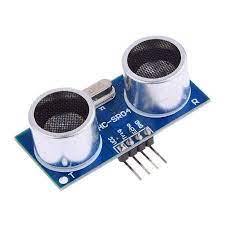
\includegraphics[scale=1]{Textuais/imagens/sensor.png}
        
        Fonte: Amazon
    \end{center}
\end{figure}

\section{Trabalhos Relacionados} \label{sec:trabrel}
Nesta seção, apresentar-se-ão exemplificações de projetos preexistentes que, até o momento, podem ou não ter sido concretizados na sociedade. Algumas das resoluções subsequentes implicam distintas metodologias, abrangendo desde a automatização das coberturas até a aplicação de Inteligência Artificial para a identificação de materiais por meio de sensores, permitindo, desse modo, a segregação dos resíduos com base em sua tipologia.


\cite{lisa} Lixeira Inteligente Seletiva Automática (LISA), entrega o projeto de uma lixeira inteligente que separa por materiais o lixo jogado nele. Os sensores são os responsáveis por detectar o material do lixo jogado e enviar informações via \textit{bluetooth} e a placa utilizada é o Arduino UNO.

 \begin{figure}[H]
    
    \label{fig:lisa}
    \begin{center}
        
        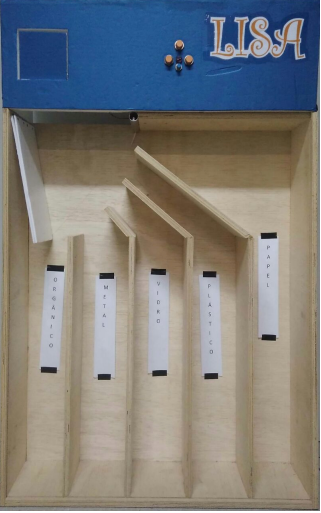
\includegraphics[scale=0.5]{Textuais/imagens/lisa.png}
        
        Fonte: \cite{lisa}
    \end{center}
\end{figure}

\cite{gaia}, o projeto GAIA apresenta a ideia de um robô inteligente que fará o trabalho de separar o lixo por categorias: plástico, vidro, papel e metal. Trata-se de um braço robô que possui uma câmera que detecta o \textit{ID} determinado por cada material e faz a separação necessária colocando o lixo em seu compartimento determinado.

 \begin{figure}[H]
    \label{fig:gaia}
    \begin{center}
        
        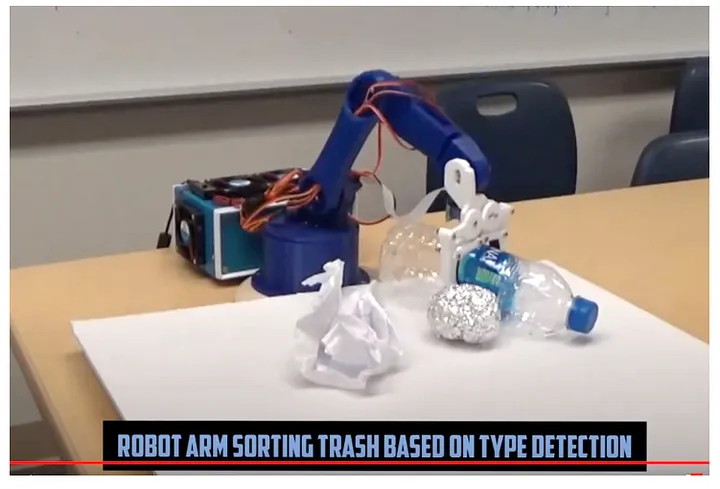
\includegraphics[scale=0.5]{Textuais/imagens/gaia.png}
        
        Fonte: \cite{gaia}
    \end{center}
\end{figure}

\cite{smartbin},  os principais locais onde o projeto pode ser instalado são os locais como shoppings, aeroportos, cinemas etc.  O projeto SmartBin é de fácil utilização e possui boa eficiência, existe a separação por 4 categorias, plástico, vidro, papel e metal. A tecnologia de espectroscopia infravermelha que é responsável pela classificação desses materiais.

 \begin{figure}[H]
    
    \label{fig:smartbin}
    \begin{center}
        
        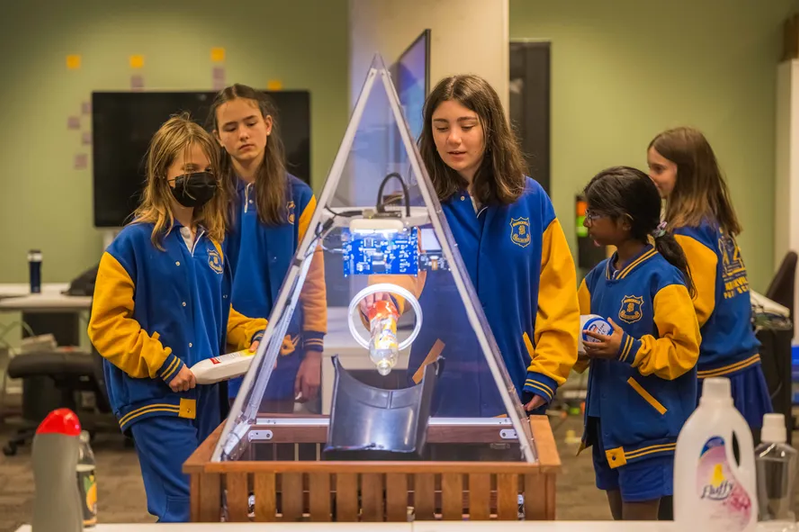
\includegraphics[scale=0.5]{Textuais/imagens/smart.png}
        
        Fonte: \cite{smartbin}
    \end{center}
\end{figure}




\section{Metodologia}

\subsection{Fases do Projeto}
O primeiro passo do projeto foi demarcado com a definição do tema, que teve origem em conversas com o professor Dr.André Luis Meneses Silva e em pesquisas realizadas. Após essa fase, iniciamos uma pesquisa e estudos acerca da plataforma \href{https://wokwi.com/}{Wokwi}, para a implementação dos módulos e códigos utilizados na \textit{Raspberry Pi}, para a lacração, limpeza da lixeira e futuramente da \textit{Inteligência artificial} (paralelo ao desenvolvimento, será feito a escrita no TCC 2) para a separação automática do lixo. Após isso, foi feita a pesquisa de trabalhos relacionados na área da modelagem de \textit{hardware} e \textit{software}. E então, foi feito um levantamento bibliográfico sobre os assuntos relacionados ao projeto como: IoT, microcontroladores, sensores, atuadores,  microcomputadores e inteligência artificial.

O segundo passo foi a análise de custo de construção e instalação da lixeira, ao qual foram analisados diversos módulos, porém apenas selecionados os que formassem um conjunto de aparelhos que realizassem o esperado e de forma barateada, melhorando o custo benefício de aquisição da lixeira. Por fim, será encaixado os aparelhos nos devidos locais, valendo ressaltar que a \textit{válvula solenóide} de escoamento deve ser implantada na parte de baixo para gerar um efeito centrífuga na água, e a de bombeamento na parte lateral para melhorar a eficiência da limpeza.

\subsection{Implementação do Projeto}
Para com a implementação e design do projeto usamos uma raspberry pi, que será usada para controlar os dados de leitura dos 2 (dois) HC-SR04, que serão instalados uma na camada inferior da parte de dentro da tampa, e outra na camada superior da parte de dentro da base da lixeira, ao qual a primeira servirá com o intuito de verificar o quão cheia está a sacola de lixo, e assim que verificado que está cheia o servo motor irá operar o mecanismo de amarração de fita à sacola de lixo. Já a segunda HC-SR04, servirá com o intuito de verificar a existência de uma sacola. Atrelado a raspberry pi terá também uma bomba de água, que irá receber o sinal da segunda HC-SR04, fazendo ou não o bombeamento da água ligado diretamente a encanação, a qual puxará a água diretamente da fonte, e fará o descarte da água residual no esgoto por meio das encanações. Isto, utilizando de 2 (duas) válvulas solenoides, para controlar o fluxo de água passada pela bomba de água, a primeira será utilizada com o intuito de abertura para o enchimento de água na lixeira, já a segunda para o esvaziamento da água contaminada.

\subsection{Recursos}
Os recursos que serão utilizados para o desenvolvimento do projeto estão relacionados ao hardware necessário e ao ambiente de desenvolvimento de código. O hardware necessário será dois microcontroladores HC-SR04 que foram apresentados na Figura \ref{fig:sensor}, um servo motor que foi apresentado na Figura \ref{fig:servomotor}, duas válvula solenóide que foram apresentadas na Figura \ref{fig:válvula selenóide}, uma bomba de água que foi apresentada na Figura \ref{fig:bomba}, os quais serão acoplados a uma Raspberry pi. Fora a necessidade da ligação as tubulações para a limpeza e descarte da água residual, além de uma polia para realizar a rotação do servo motor com a fita.

\subsection{Avaliação do Impacto Social}
Como avaliação do impacto social, é analisado sobre como a lixeira inteligente irá impactar no âmbito social, na boa relação entre os grandes centros urbanos e o meio ambiente e em como a falta do tratamento devido traz à tona prejuízos para todos os seres vivos e não vivos. 

A priori, a redução do mau odor das lixeiras é uma medida fundamental para melhorar a qualidade de vida e o bem-estar das pessoas, bem como para minimizar os impactos negativos nos animais que vivem nas proximidades. Além da limpeza constante, o uso de sacos de lixo resistentes e à prova de vazamentos pode ajudar a conter os odores desagradáveis provenientes da mistura de materiais orgânicos e inorgânicos. Outra estratégia eficaz envolve o armazenamento adequado dos resíduos, como o uso de recipientes herméticos, que evitam a disseminação dos odores. Essas práticas não apenas reduzem o mau odor, mas também contribuem para manter a higiene e a saúde das comunidades, criando um ambiente mais agradável e saudável para todos. Além disso, ao minimizar o mau odor, reduz-se o risco de atração de pragas, como insetos e roedores, que podem representar problemas adicionais de saúde e segurança. Portanto, o cuidado com a gestão de resíduos e a mitigação dos odores desagradáveis são aspectos cruciais do gerenciamento de resíduos em áreas urbanas e rurais.

A posteriori, surge a necessidade de lidar com a secreção causada pela falta da higienização adequada aos lixos, que é o chorume. Tal líquido é tanto nocivo para os seres vivos que entram em contato, quanto para com a contaminação de lençóis freáticos e poços artesianos nos centros urbanos. Em relação aos animais, que entram em contato com líquido tóxico que se forma a partir da decomposição de resíduos orgânicos, sofrem com o  envenenamento. Além disso, o vazamento de chorume pode contaminar o solo e as fontes de água próximas, destruindo habitats naturais e tornando esses ambientes inadequados para a vida selvagem. Já em relação aos humanos, a contaminação do chorume nos lençóis freáticos e poços artesianos representa uma séria ameaça à qualidade da água potável. O chorume, ao infiltrar-se nessas fontes subterrâneas, pode poluir a água com substâncias tóxicas, tornando-a inadequada para consumo humano. Isso coloca em risco a saúde.

\subsection{Detalhamento}
 \begin{figure}[H]
    \caption{Imagem do Circuito do projeto}
    \label{fig:sensor}
    \begin{center}
        
        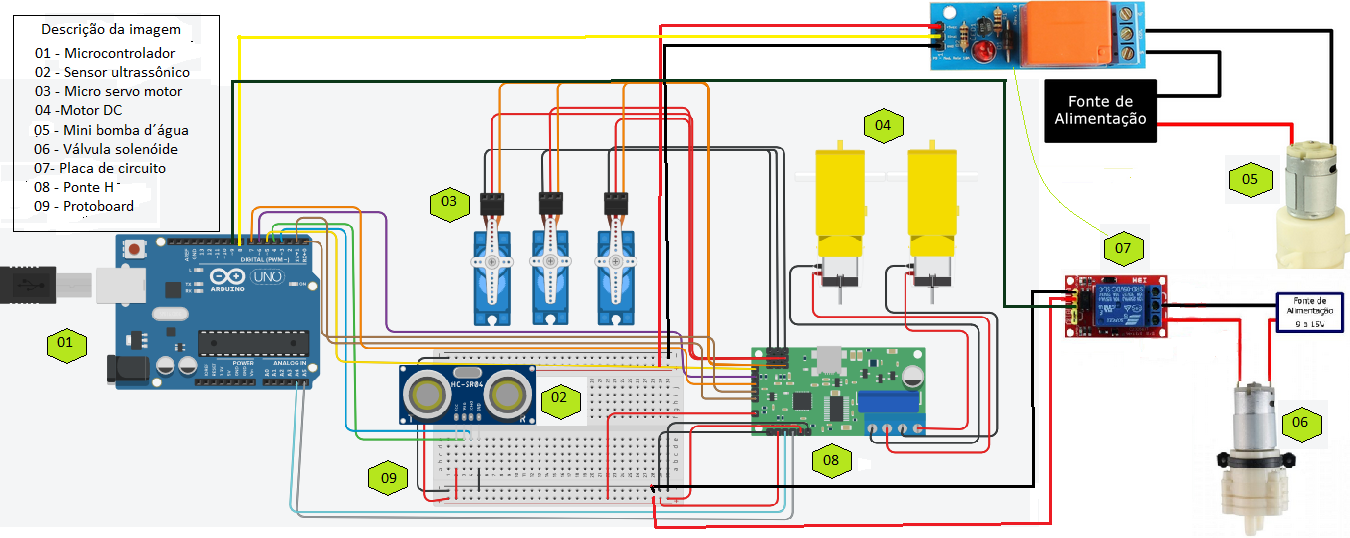
\includegraphics[scale=0.5]{circuito.png}
        
        Fonte: Autoria própria
    \end{center}
\end{figure}

A Figura 6 é um pequeno esboço do projeto, numa visão do hardware que o compõe e suas conexões. Na criação dessa figura foi utilizado o software Thinkercad e posteriormente editada a imagem no paint. Na imagem temos Arduino que fará o papel de microcontrolador, também temos três micro servos motores e dois motores DC ligados a uma ponte h que está conectada ao Arduino. Temos também uma bomba d'água ligadas numa placa de circuito que está conectada ao Arduino e uma válvula solenoide ligada a uma placa de circuito e conectada ao Arduino.

A lixeira irá possuir na frente um painel, nesse caso, um tablet para usuário informar qual o lixo que deseja descartar. Após o usuário informar qual o tipo de lixo ele deseja descartar a lixeira se abre e a tela solicita que o usuário deposite o lixo especificado.

Dentro da lixeira há um desnível controlado por um motor que ao ser colocado o lixo ele abre o compartimento respectivo para o descarte desse lixo. Dentro do compartimento há um sensor ultrassônico na parte superior, um motor para inserir a sacola de lixo nova e lacrar a sacola de lixo cheia sempre que necessário, embaixo há um sensor de peso acoplado a uma esteira que ao alcançar o peso especificado no projeto que irá informar ao sistema que o lixo está cheio na parte inferior traseira interna de cada compartimento há um motor acoplado há uma saída por onde o saco de lixo lacrado será enviado pela esteira para um compartimento onde estará disponível para coleta e reciclagem. Para facilitar a coleta, o saco de lixo em cada compartimento deverá ter uma cor diferente de acordo com as especificações de coleta e reciclagem e assim facilitará o trabalho do coletor.

Nos compartimentos necessários, onde há materiais orgânicos e materiais que possam ser reciclados porém sujos ou que necessitam de um pré-processamento, haverá nas laterais um motor acoplado a uma bomba d'água com o mecanismo de alto limpeza evitando o mau odor do lixo e abaixo destes compartimentos teremos uma válvula solenóide na saída por onde a água suja irá por encanamento para o esgoto evitando assim a contaminação do solo.








\section{Conclusões}

Este trabalho apresentou a \textit{Lixeira Inteligente}, uma proposta que representa uma solução inovadora e promissora para a gestão eficiente de resíduos sólidos em ambientes urbanos. Ao longo deste trabalho, foram explorados diversos aspectos, desde o projeto e a implementação do \textit{hardware} e \textit{software} até a avaliação do desempenho e da viabilidade da lixeira inteligente.

O sistema foi projetado com a finalidade de otimizar a coleta, lacração e limpeza de resíduos, tornando o processo mais eficiente, higiênico e sustentável. A integração de sensores, atuadores e automação permite que a lixeira determine o nível de enchimento, execute a limpeza automática e garanta a prontidão para receber novos resíduos.

Uma das características distintivas desse projeto é a ênfase na eficiência energética, com o objetivo de minimizar o consumo de recursos e reduzir o impacto ambiental. O uso de sensores ultrassônicos HC-SR04 proporciona uma medição precisa do nível de enchimento da lixeira, enquanto a automação, controlada pela Raspberry Pi, coordena todo o processo.

Este projeto não é apenas uma resposta inovadora ao desafio da gestão de resíduos, mas também um exemplo do potencial da tecnologia para aprimorar a vida nas cidades. À medida que a urbanização continua a crescer, soluções inteligentes e sustentáveis são essenciais para enfrentar os desafios associados à expansão urbana e à preservação do meio ambiente. A lixeira automática representa um passo significativo em direção a um futuro mais limpo, eficiente e sustentável, onde a tecnologia desempenha um papel crucial na melhoria das condições de vida nas áreas urbanas e na promoção da responsabilidade ambiental. O projeto não foi concretizado mas este artigo ajudará neste procedimento, com o intuito de promover a sua concretização.



%-------------------
\bibliography{referencias}
\bibliographystyle{chicago}

\newpage
\singlespacing
\begin{center}
\bigskip
\bigskip 
\bigskip 
\bigskip 
\bigskip 
\bigskip
Itabaiana, 16 de outubro de 2023
\bigskip
\bigskip 
\bigskip 
\bigskip 
\bigskip \\ 
\rule{7cm}{0.4pt} \\
Prof. Dr. André Luis Meneses Silva \\
Assinatura do Orientador
\bigskip
\bigskip 
\bigskip \\
\rule{7cm}{0.4pt} \\
Arlene De Almeida Pereira Siqueira\\
Camila Fontes Santos\\
Laila Esterfane Dos Santos Valença\\
Marlysson Silva Dantas\\
Miguel Ferreira França\\
Vinicius Lima Santos \\
Assinatura do Aluno
\end{center}


\end{document}
